
\section{Backend Development}

\subsection{Backend Architecture with ASP.NET Core}
The backend services were developed using ASP.NET Core, which enabled the creation of secure, scalable APIs. This layer handles user authentication, data management, and integration with controllers. Key elements include:
\begin{itemize}
    \item \textbf{API Development}: Exposing endpoints for frontend communication using controllers in ASP.NET.
    \item \textbf{Security Measures}: Implementation of token-based authentication and authorization to protect sensitive data.
    \item \textbf{Data Management}: Interaction with a SQL Server database to store and retrieve information.
\end{itemize}

\subsection{Database Structure}
The database schema was designed to handle the various entities within the LAB.E.S system, including:
\begin{itemize}
    \item \textbf{Equipment Data}: Information about laboratory instruments and their configurations.
    \item \textbf{Test Records}: Data related to different tests performed, linked to equipment and users.
    \item \textbf{User Management}: Storing user profiles, access levels, and activity logs.
\end{itemize}
\begin{figure}[H]
    \centering
    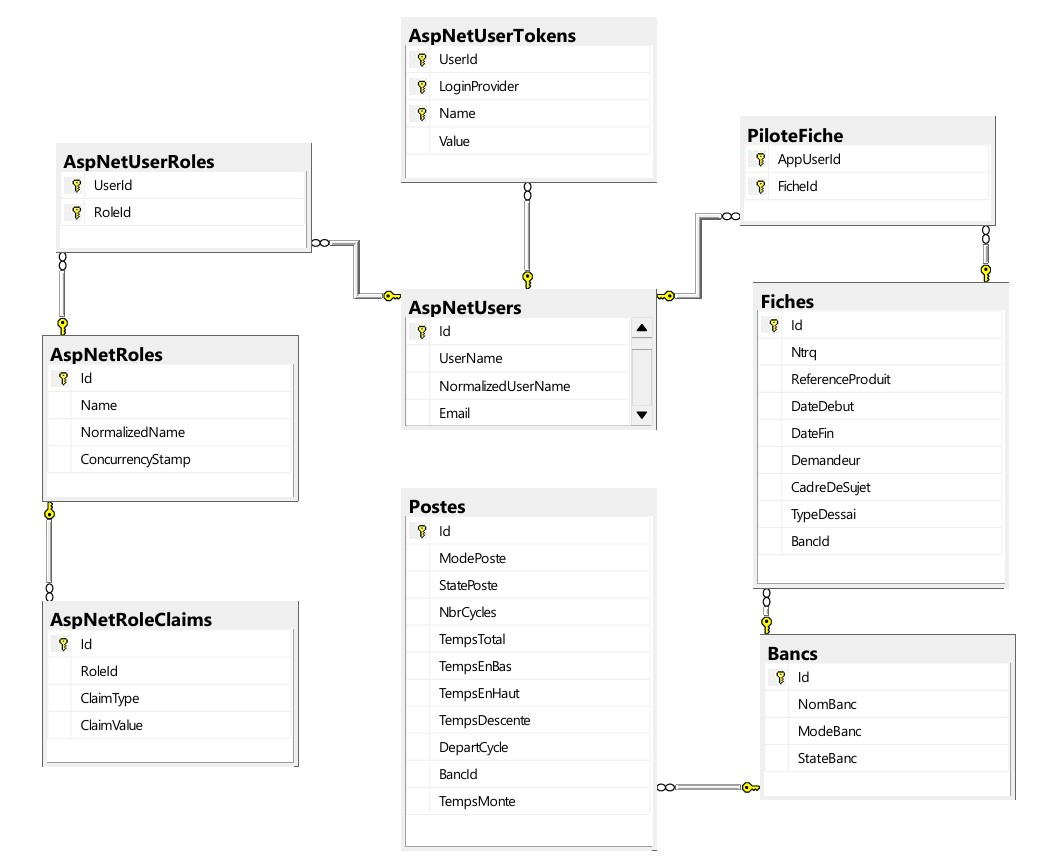
\includegraphics[width=1\textwidth]{chapters/3/img/16.jpg}
    \caption{cp 242-1 LEAN}
    \label{fig:campus}
\end{figure}


\subsection
{Services Déployés dans les iBox}
Pour récupérer les données des automates, plusieurs services ont été déployés sur les iBox :

\subsubsection{Service de Communication :} Gère les échanges de données entre les automates et les systèmes centralisés.
\subsubsection{Service de Stockage :} Assure la collecte et le stockage des données pour une analyse ultérieure.
\subsubsection{Service de Monitoring :} Surveille en temps réel les performances des automates et des flux de données.
